
\item Two spheres \( P \) and \( Q \) of equal radii have densities \( \rho_1 \) and \( \rho_2 \), respectively. The spheres are connected by a massless string and placed in liquids \( L_1 \) and \( L_2 \) of densities \( \sigma_1 \) and \( \sigma_2 \) and viscosities \( \eta_1 \) and \( \eta_2 \), respectively. They float in equilibrium with the sphere \( P \) in \( L_1 \) and sphere \( Q \) in \( L_2 \) and the string being taut (see figure). If sphere \( P \) alone in \( L_2 \) has terminal velocity \( \vec{V}_P \) and \( Q \) alone in \( L_1 \) has terminal velocity \( \vec{V}_Q \), then
        \begin{tasks}(2)
            \task \( \left| \vec{V}_P \right| / \left| \vec{V}_Q \right| = \eta_1 / \eta_2 \)
            \task \( \left| \vec{V}_P \right| / \left| \vec{V}_Q \right| = \eta_2 / \eta_1 \)
            \task \( \vec{V}_P \cdot \vec{V}_Q > 0 \)
            \task \( \vec{V}_P \cdot \vec{V}_Q < 0 \)
        \end{tasks}
\begin{center}
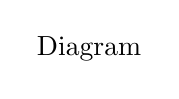
\begin{tikzpicture}
\node {Diagram};
\end{tikzpicture}
\end{center}
